\documentclass[aspectratio=169]{beamer}
\usetheme{CambridgeUS}
\usecolortheme{spruce}
\setbeamersize{text margin left=1cm,text margin right=1cm}
\usepackage[utf8]{inputenc}
\usepackage[T1]{fontenc}
\usepackage[czech]{babel}
\usepackage{csquotes}
\usepackage{amsmath}
\usepackage{tikz}
% \usefonttheme{professionalfonts}
\usetikzlibrary{%
 positioning, graphs, graphs.standard, shapes.geometric,quotes, calc, perspective, shapes, arrows.meta
}
\usepackage{pgfplots}
\usepackage{tikz-3dplot}
\usepackage{caption}
\usepackage{subcaption}
\pgfplotsset{compat=1.18}
\usepackage{svg}
\definecolor{myred}{RGB}{170, 55, 55}
\definecolor{myblue}{RGB}{88,118,199}
\definecolor{mygreen}{RGB}{74, 108, 145}
\definecolor{graph}{RGB}{102,138,224}
\definecolor{graph2}{RGB}{224,102,138}
\definecolor{myorange}{RGB}{237, 120, 36}


\definecolor{green1}{RGB}{30, 58, 86}
\definecolor{green2}{RGB}{74, 108, 145}
\definecolor{green3}{RGB}{141, 165, 195}

\definecolor{white1}{RGB}{220,250,250}
\definecolor{vyzkum_color}{RGB}{119,96,210}

\setbeamercolor{structure}{fg=mygreen} % Change the color of structural elements to "myred"
% \setbeamercolor{block title}{bg=mygreen2, fg=white} % Change the color of block titles
\setbeamercolor{block title}{bg=myblue, fg=white}

\setbeamercolor{palette primary}{bg=green1}
\setbeamercolor{palette secondary}{bg=green2}
\setbeamercolor{palette tertiary}{bg=green3}
\setbeamercolor{frametitle}{bg=green2, fg=white}

\setbeamercolor{title in head/foot}{fg=white1}
\setbeamercolor{author in head/foot}{fg=white1}
\setbeamercolor{date in head/foot}{fg=white1}
\setbeamercolor{title}{fg=white}
\setbeamercolor{section in head/foot}{fg=white1}
\setbeamercolor{subsection in head/foot}{fg=white1}

\newenvironment<>{vyzkum}[1]{%
  \setlength{\textwidth}{1\textwidth}
  \setbeamercolor{block title}{fg=white,bg=vyzkum_color}%
  \begin{block}#2{#1}}{\end{block}}
\newenvironment<>{random}[1]{%
    \setlength{\textwidth}{0.75\textwidth}
    \setbeamercolor{block title}{fg=white,bg=green1}%
    \begin{block}#2{#1}}{\end{block}}

\newenvironment<>{informace}[1]{%
    \setlength{\textwidth}{1\textwidth}
    \setbeamercolor{block title}{fg=white,bg=myblue}%
    \begin{block}#2{#1}}{\end{block}}

\newenvironment<>{otazka}[1]{%
    \setlength{\textwidth}{1\textwidth}
    \setbeamercolor{block title}{fg=white,bg=myorange}%
    \begin{block}#2{#1}}{\end{block}}

\usepackage{enumitem,amssymb}
\newlist{todolist}{itemize}{2}
\setlist[todolist]{label=$\square$}
\usepackage{pifont}
\newcommand{\cmark}{\ding{51}}%
\newcommand{\xmark}{\ding{55}}%
\newcommand{\done}{\rlap{$\square$}{\raisebox{2pt}{\large\hspace{1pt}\cmark}}%
\hspace{-2.5pt}}
\newcommand{\wontfix}{\rlap{$\square$}{\large\hspace{1pt}\xmark}}

\newtheorem{definice}{Definice}
\newcommand{\R}{\mathbb{R}}
\beamertemplatenavigationsymbolsempty
\title[IVT]{Externí paměť}
\author{Eric Dusart}
\date{\today}

\begin{document}

\frame{\titlepage}

\begin{frame}
  \tableofcontents
\end{frame}

\section{Fonograf}
\begin{frame}
  \frametitle{Fonograf (1877)}
  \begin{minipage}{0.65\textwidth}
    \begin{itemize}[label=\textbullet]
      \item Thomas Edison.
      \item První přístroj na nahrávání a reprodukci hlasu.
      \item Váleček z kovu se spirálovou drážkou a jehlou pokrytý voskem.
    \end{itemize}
  \end{minipage}%
  \begin{minipage}{0.35\textwidth}
    \begin{figure}
      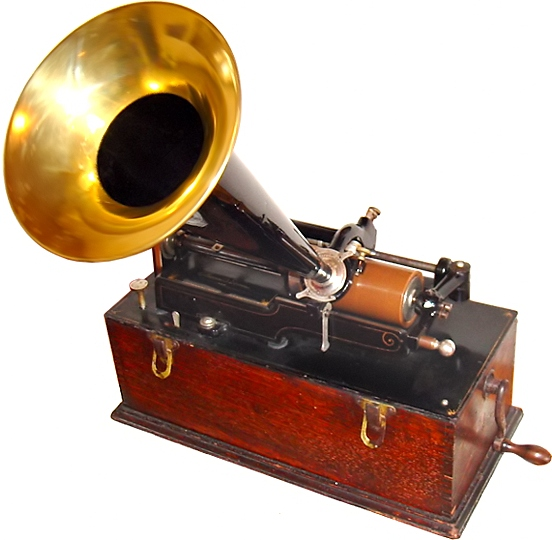
\includegraphics[width=\textwidth]{d}
      \caption{Fonograf}
    \end{figure}
  \end{minipage}
\end{frame}

\section{Magnetické paměti}
\subsection{Magnetická páska}
\begin{frame}
  \frametitle{Magnetická páska $1926$ (zvuk), $1951$(data)~-~$\approx 2010$ }
  \begin{minipage}{0.65\textwidth}
    \begin{itemize}[label=\textbullet]
      \item Plastová páska s magnetickou vrstvou.
      \item Nejprve sloužily k záznamu zvuku, poté i k záznamu videa a k uchovávání dat.
      \item Zvuk se mohl stříhat.
      \item Médium se sekvenčním přístupem.
      \item Nevýhody:
      \begin{itemize}[label=\textbullet]
        \item Páska se musela přetáčet.
        \item Některé pásky mohou trpět tzv. syndromem rozpadu pojiva.
      \end{itemize}
      \item Výhody:
      \begin{itemize}[label=\textbullet]
        \item Levná cena.
        \item Dlouhá životnost, degradace po 10 až 20 letech.
        \item Může být i velké úložiště.
      \end{itemize} 
    \end{itemize}
  \end{minipage}%
  \begin{minipage}{0.35\textwidth}
    \begin{figure}
      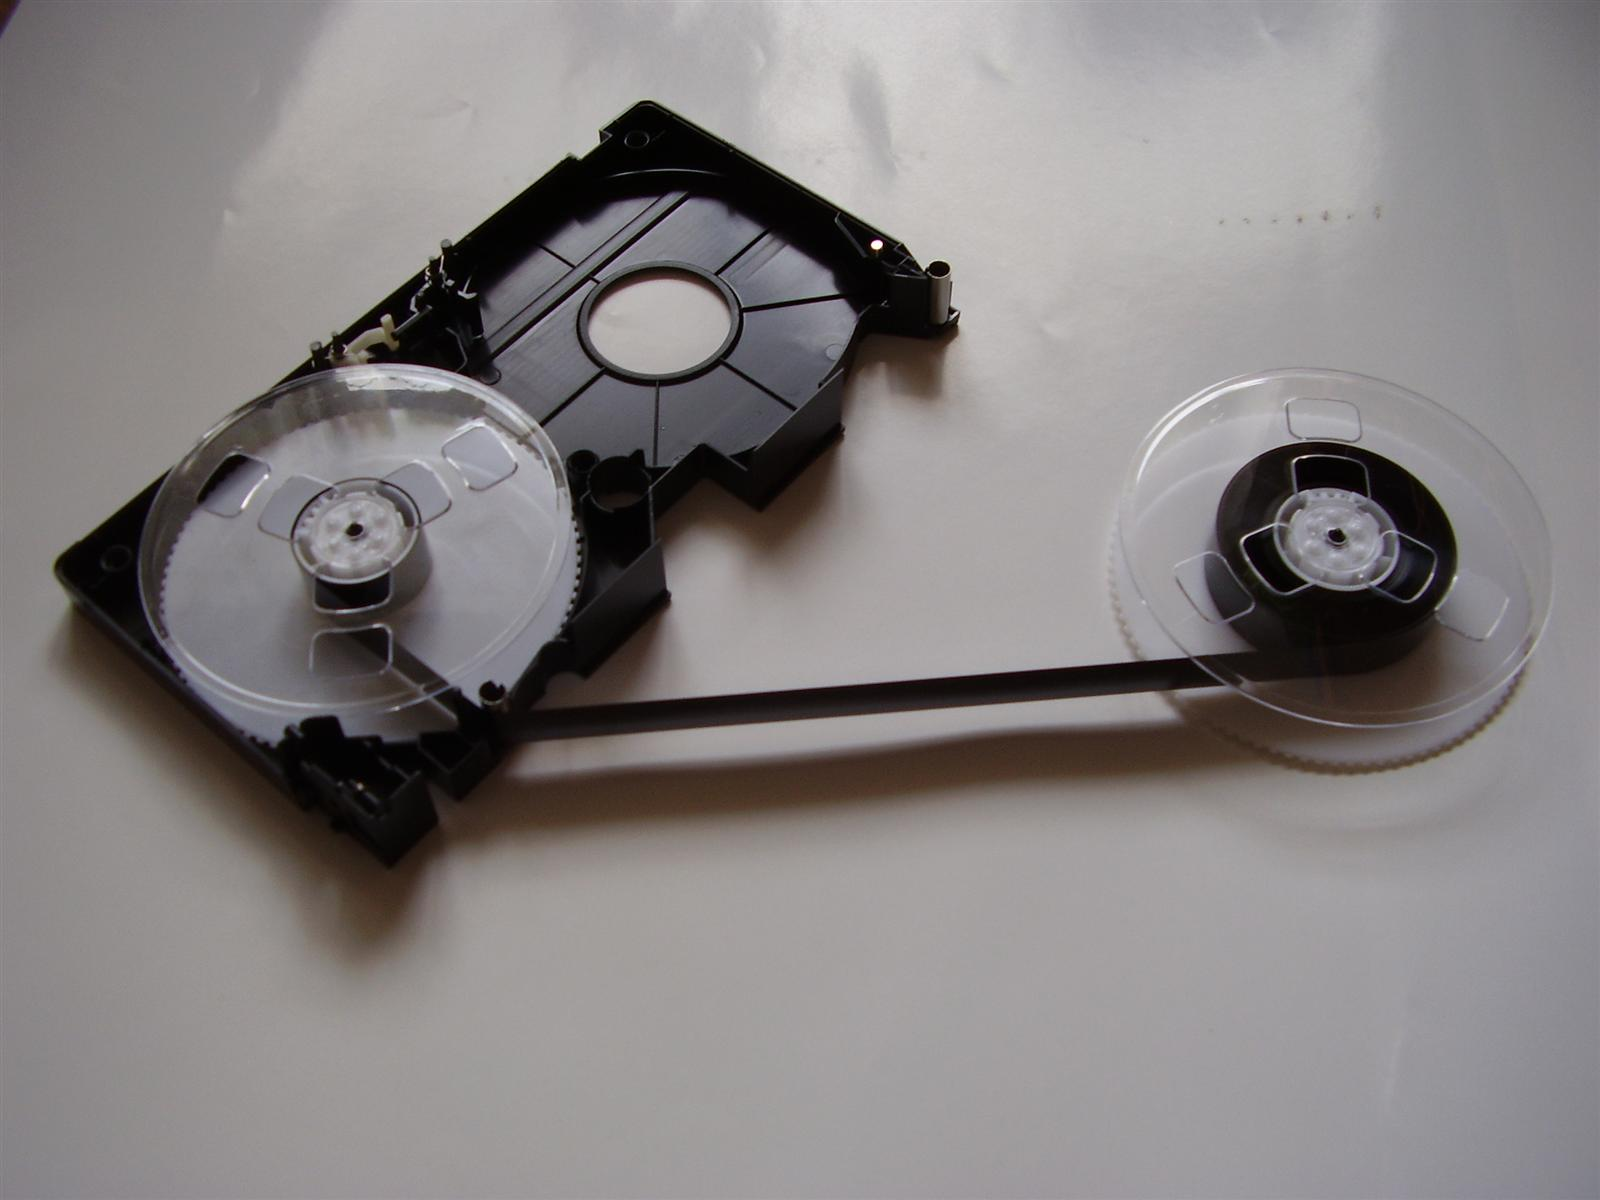
\includegraphics[width=\textwidth]{a}
    \caption{\href{https://youtu.be/lRNv4uM6auI?t=593}{Kazeta}}
    \end{figure}
    
  \end{minipage}
\end{frame}

\subsection{Floppy disk}
\begin{frame}
  \frametitle{Diskety (Floppy disky) $ 1970~-~\approx 2010$}
  \begin{minipage}{0.65\textwidth}
    \begin{itemize}[label=\textbullet]
      \item Zase založené na magnetickém principu.
      \item Levné, proto byly populární.
      \item Ikona uložení souborů.
      \item Jsou ohybné / pružné.
    \end{itemize}
    \begin{table}
      \centering
      \begin{tabular}{|c|c|c|c|}
        \hline
        \textbf{Průměr} & \multicolumn{3}{|c|}{\textbf{Kapacita}}\\ 
        \hline
        8\,\text{''} & 160 KiB & 512 KiB & 1.2 MiB \\
        \hline
        5.25\,\text{''} & 360 KiB & 720 KiB & 1.2 MiB \\
        \hline
        3.5\,\text{''} & 720 KiB & 1.44 MiB & 2.88 MiB \\
        \hline
      \end{tabular}
      \caption{Evoluce Floppy disků}
    \end{table}
  \end{minipage}%
  \begin{minipage}{0.35\textwidth}
    \begin{figure}
      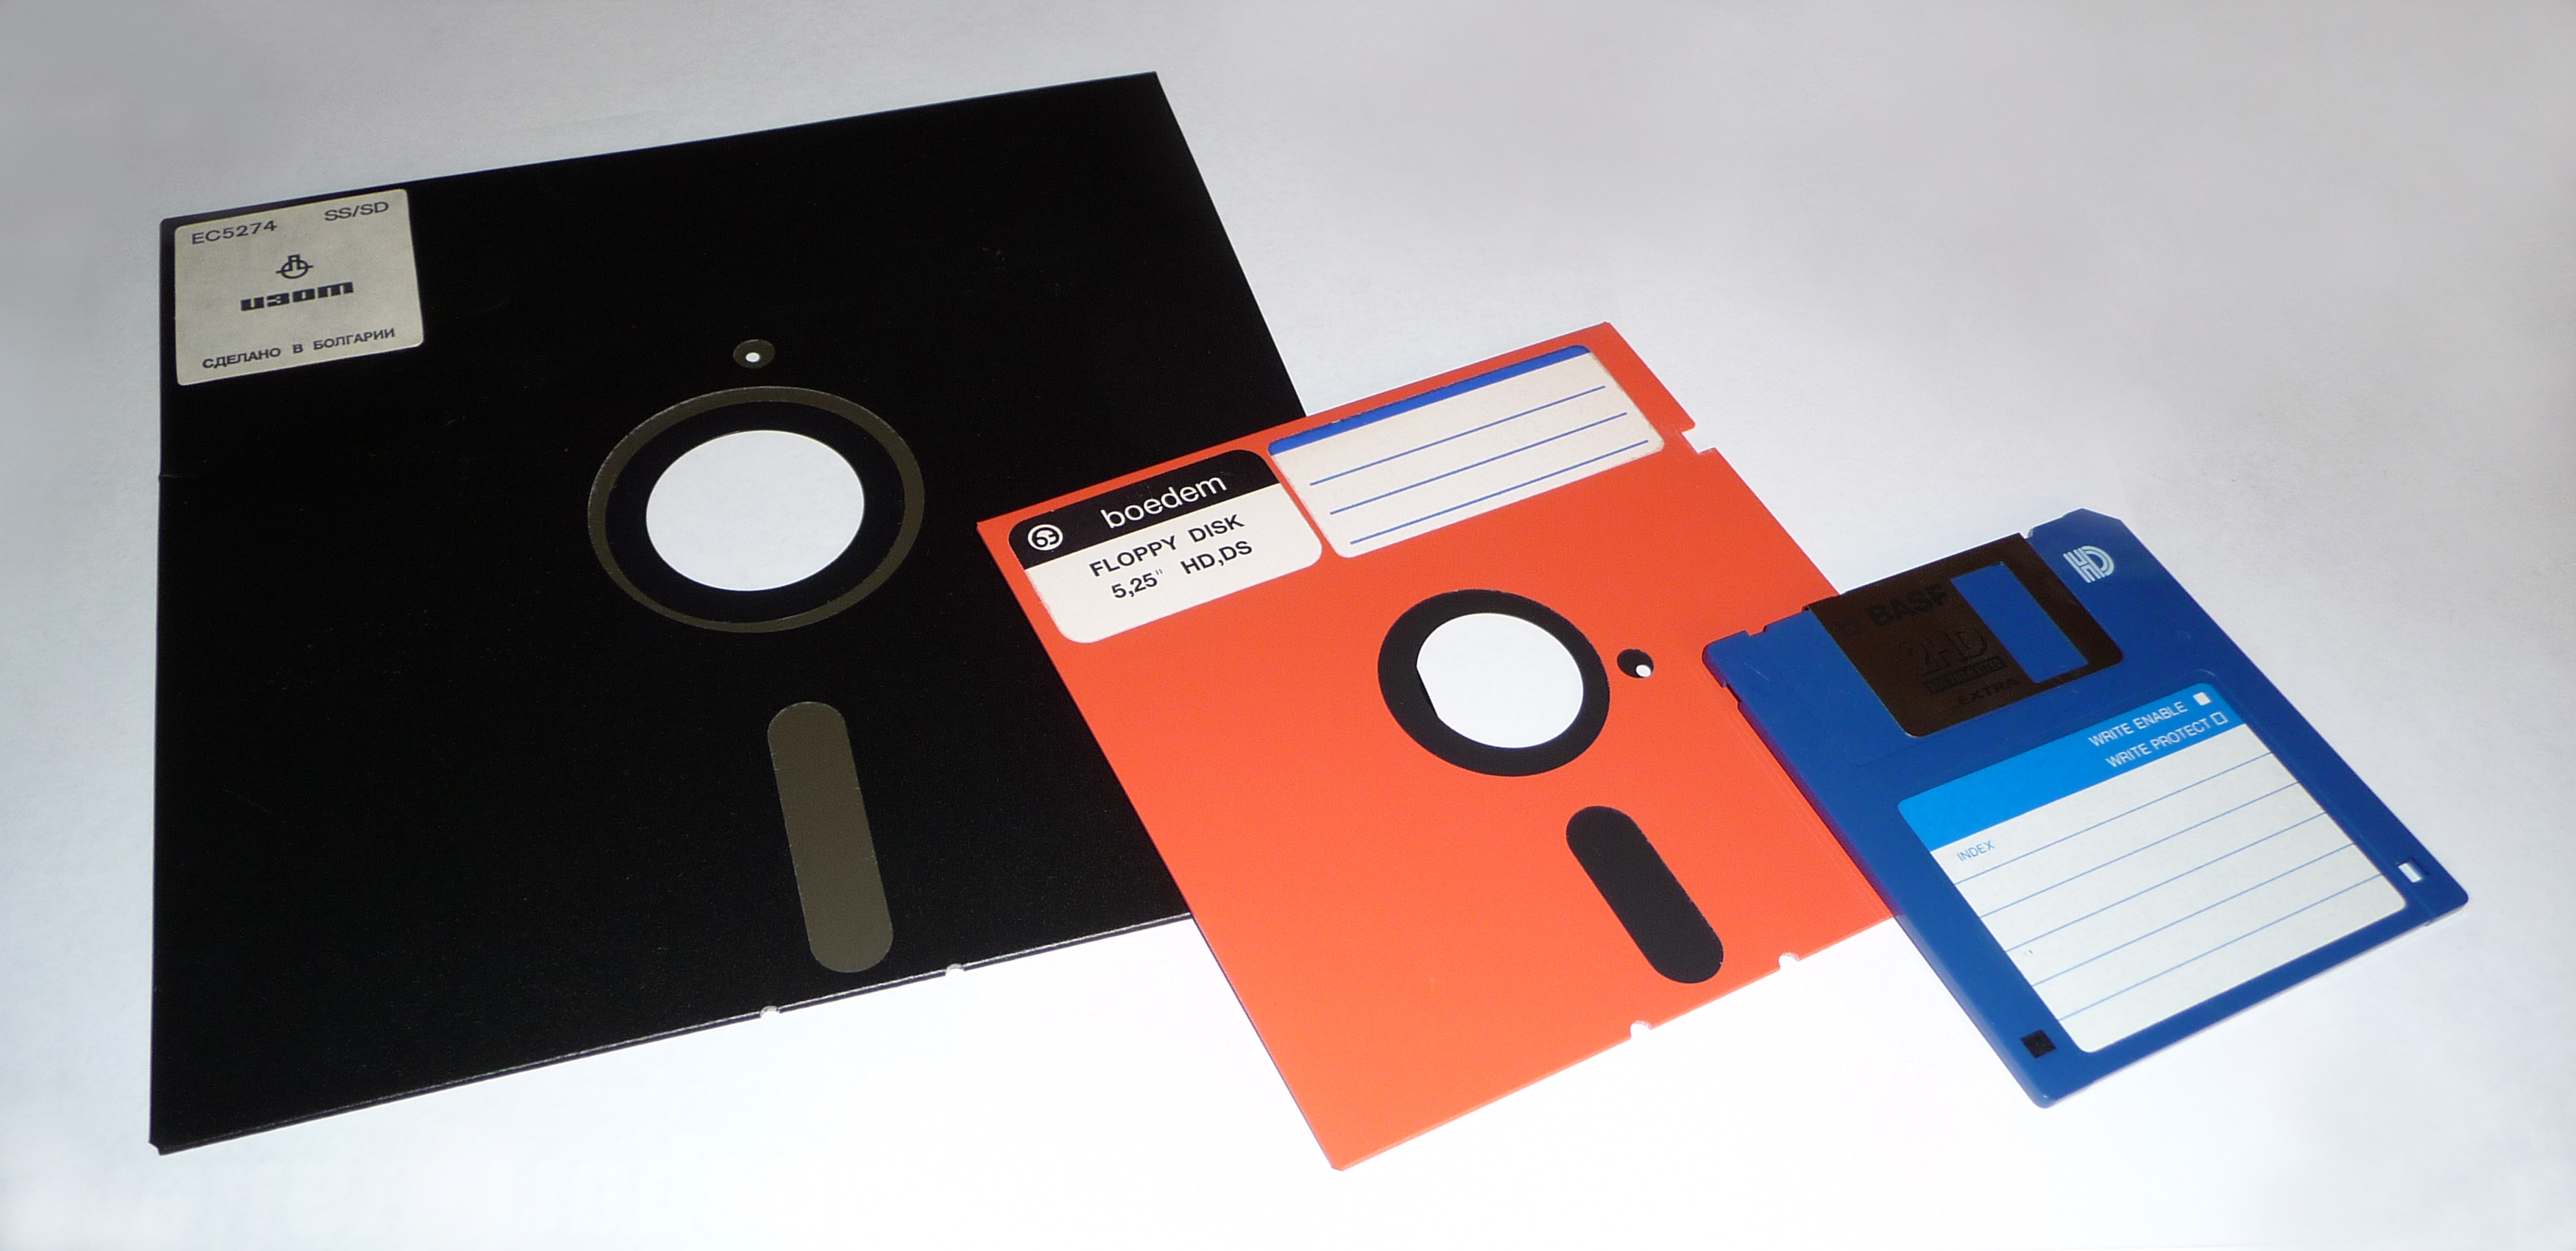
\includegraphics[width=\textwidth]{b}
      \caption{Floppy disky}
    \end{figure}
    \vspace{-0.5cm}
    \begin{figure}
      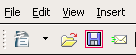
\includegraphics[width=\textwidth]{c}
      \caption{Floppy disky}
    \end{figure}
    
  \end{minipage}
\end{frame}

\begin{frame}
  \begin{figure}
    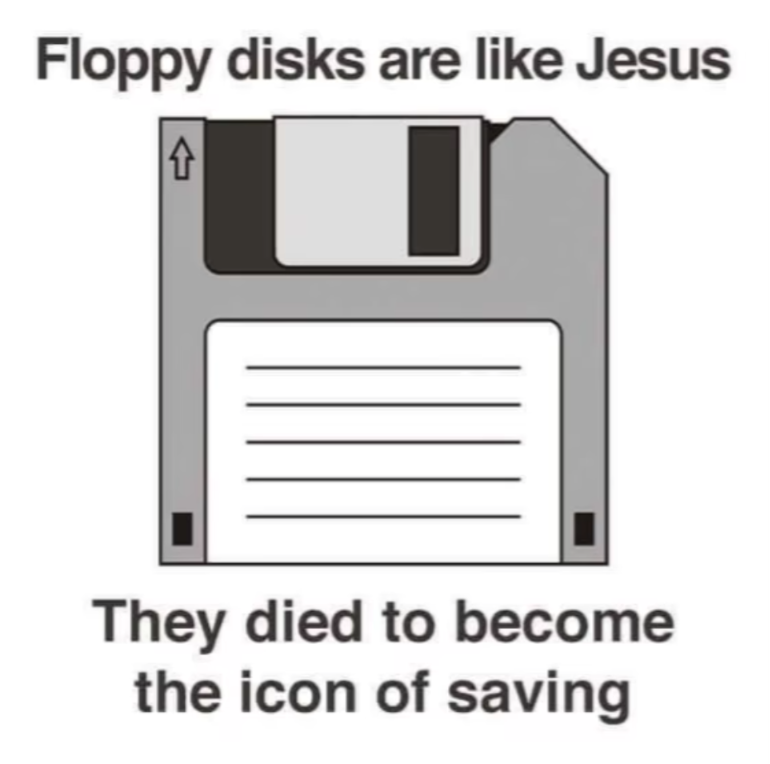
\includegraphics[width=0.5\textwidth]{l}
    \caption{meme}
  \end{figure}
\end{frame}

\begin{frame}
  \begin{figure}[t]
    \centering
    \begin{minipage}[t]{0.45\textwidth}
      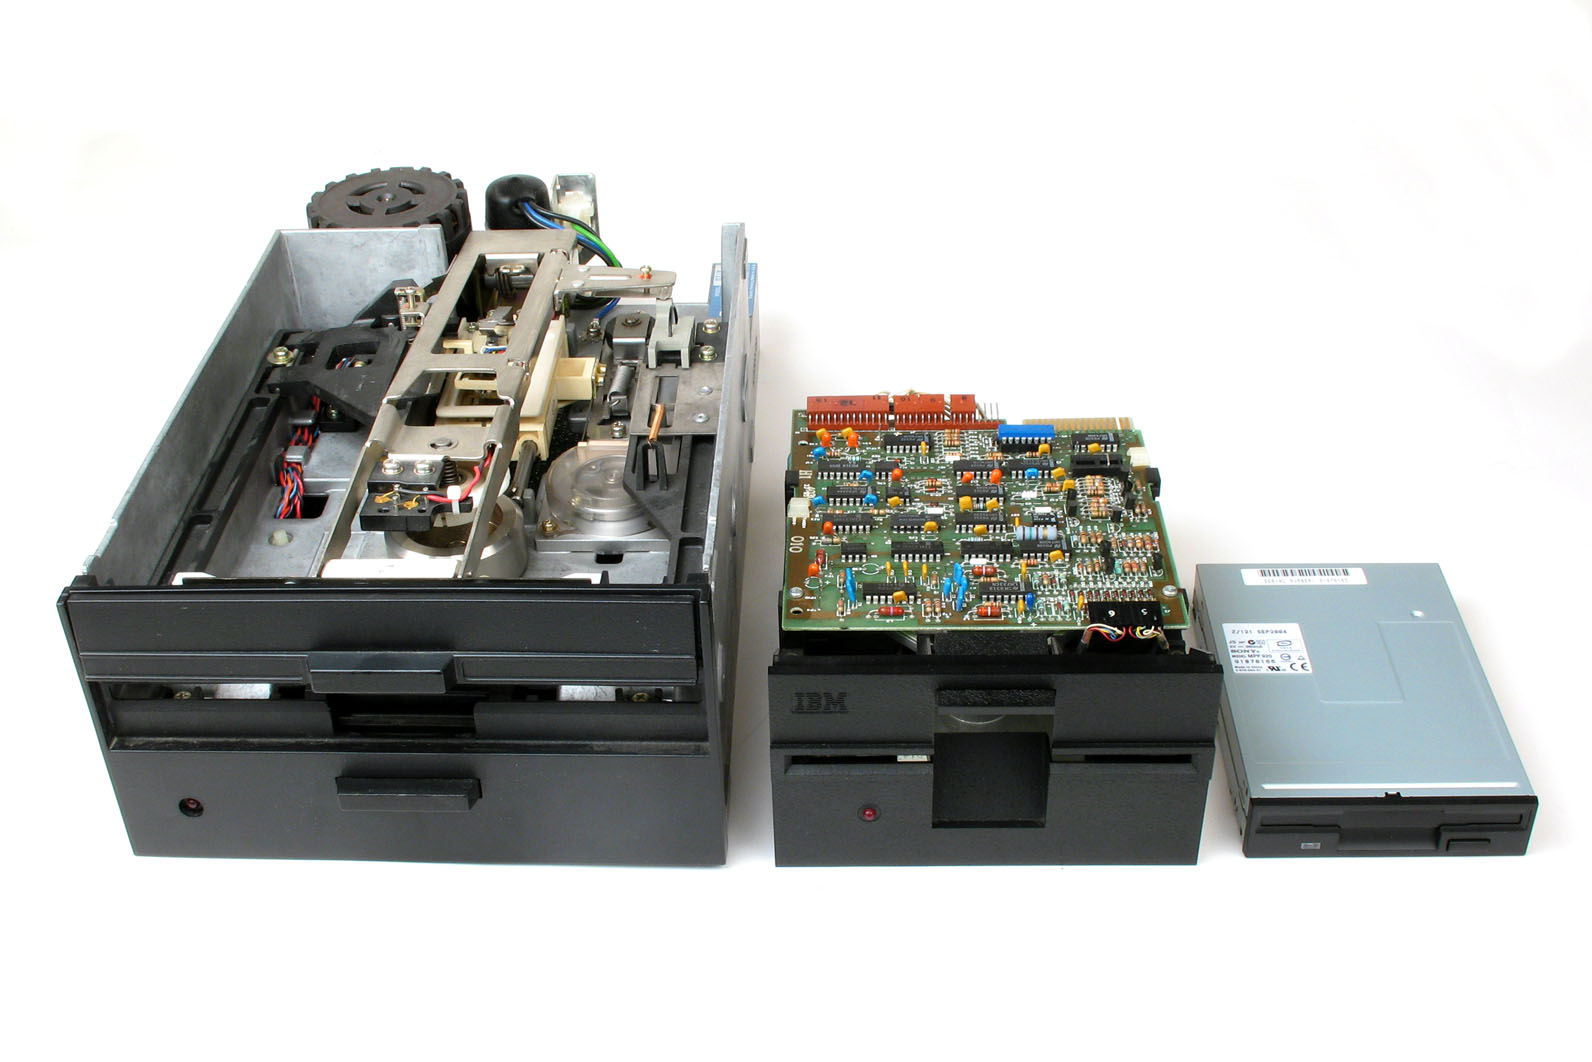
\includegraphics[width=\textwidth]{e}
      \caption{Disketové mechaniky}
    \end{minipage}
    \hfill
    \begin{minipage}[t]{0.45\textwidth}
      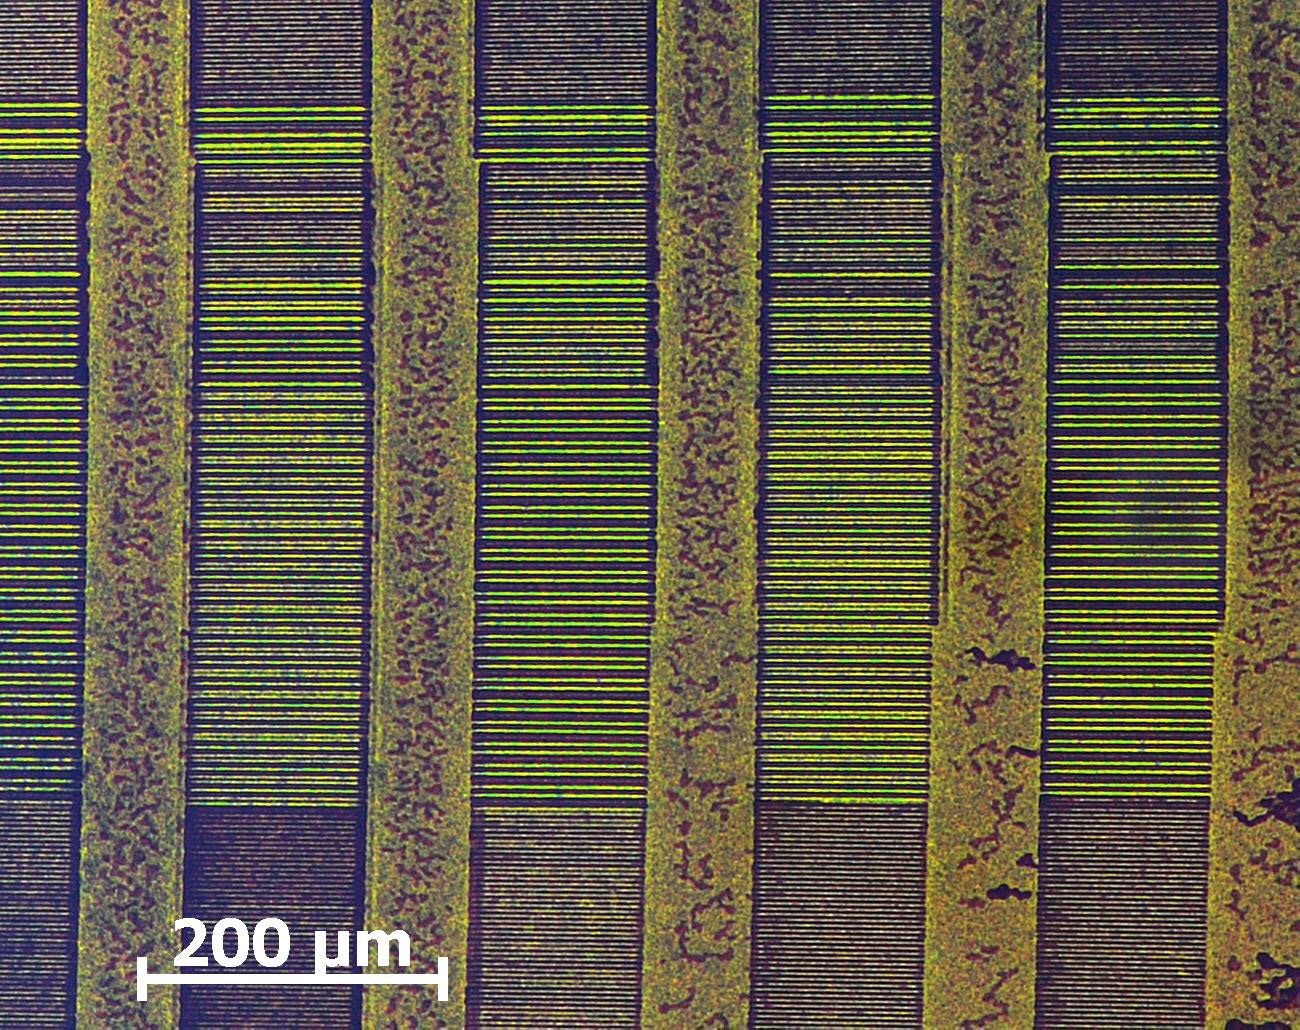
\includegraphics[width=\textwidth]{f}
      \caption{Magnetické informace na disketě}
    \end{minipage}
  \end{figure}
\end{frame}

\begin{frame}
    \begin{itemize}[label=\textbullet]
      \item Jak probíhá zapisování:
      \begin{itemize}[label=\textbullet]
        \item Disk se točí.
        \item Hlava magnetizuje povrch disku a otáčí částice na jednu nebo druhou stranu podle magnetického pólu. Tím se zaznamená binární kód.
      \end{itemize}
    \end{itemize}
    \begin{figure}
      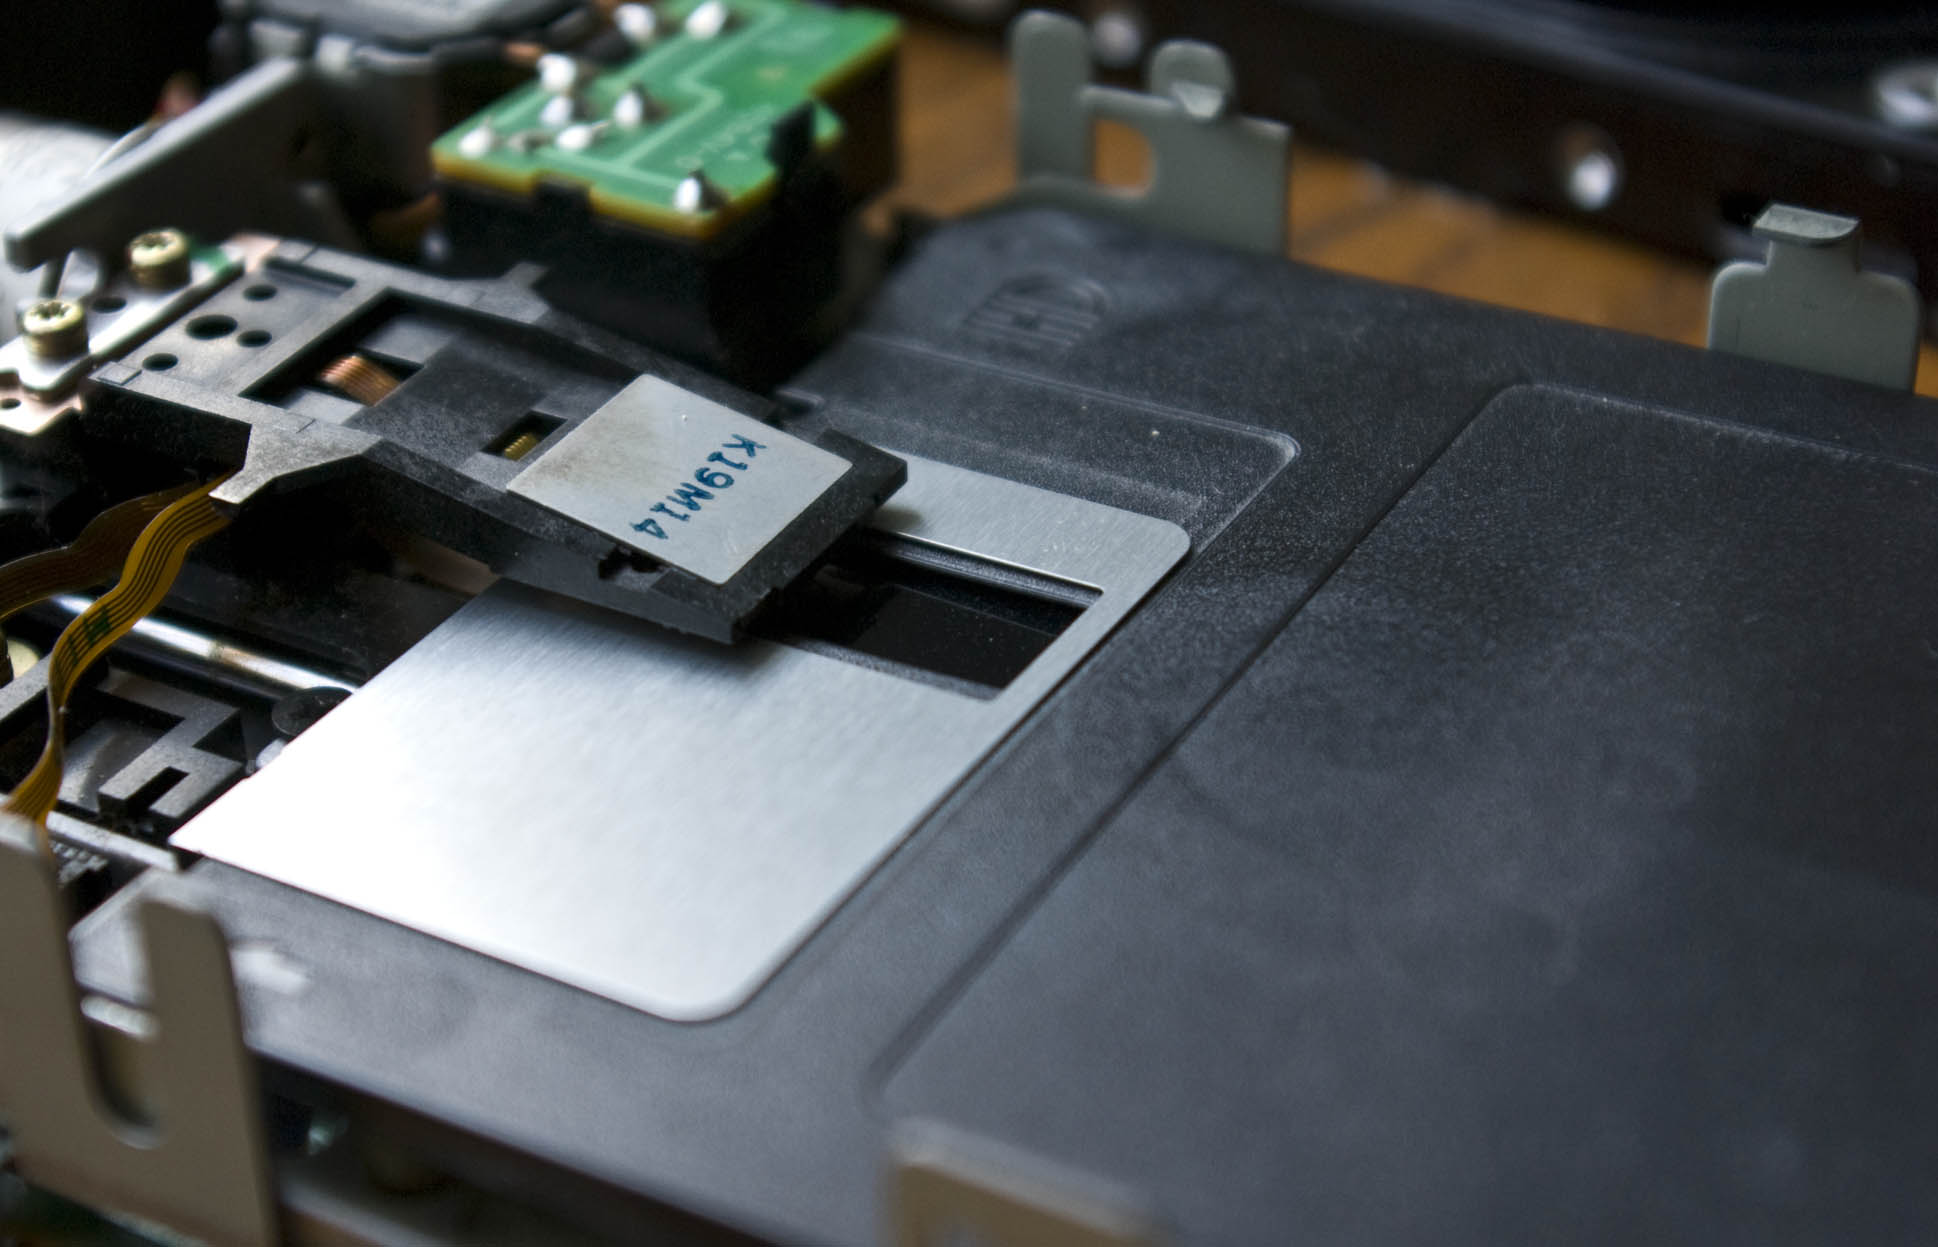
\includegraphics[width=0.5\textwidth]{g}
      \caption{Čtecí a zapisovací hlava}
    \end{figure}
\end{frame}
\subsection{HDD}
\begin{frame}
  \frametitle{Pevný disk (HDD) - 1956 (IBM)}
  \begin{minipage}{0.5\textwidth}
    \begin{itemize}[label=\textbullet]
      \item Magnetický princip.
      \item Random access.
      \item Asi nejvíce vylepšený za celou dobu.
      \item 3.5-inch, 2.5-inch.
    \end{itemize}
    \hfill
  \end{minipage}
  \hfill
  \begin{minipage}{0.45\textwidth}
    \begin{figure}
      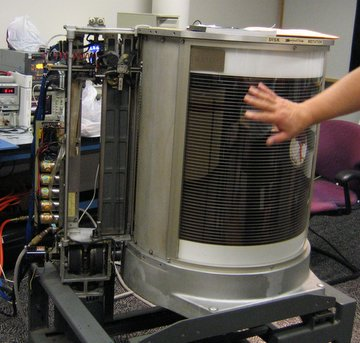
\includegraphics[width=\textwidth]{m}
      \caption{IBM 350 RAMAC, Kapacita 5Mb}
    \end{figure}
  \end{minipage}
\end{frame}
\begin{frame}
  \centering
  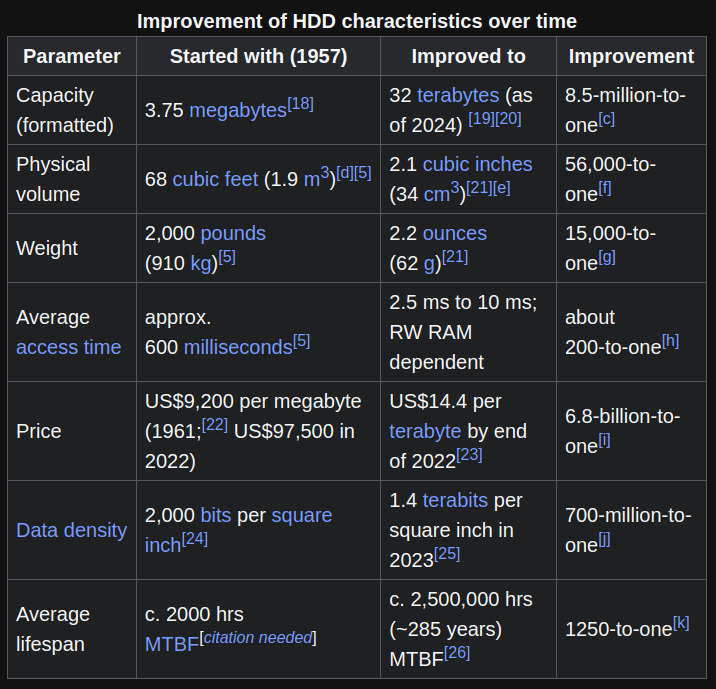
\includegraphics[width=0.6\textwidth]{n}
\end{frame}
\begin{frame}
  \centering
  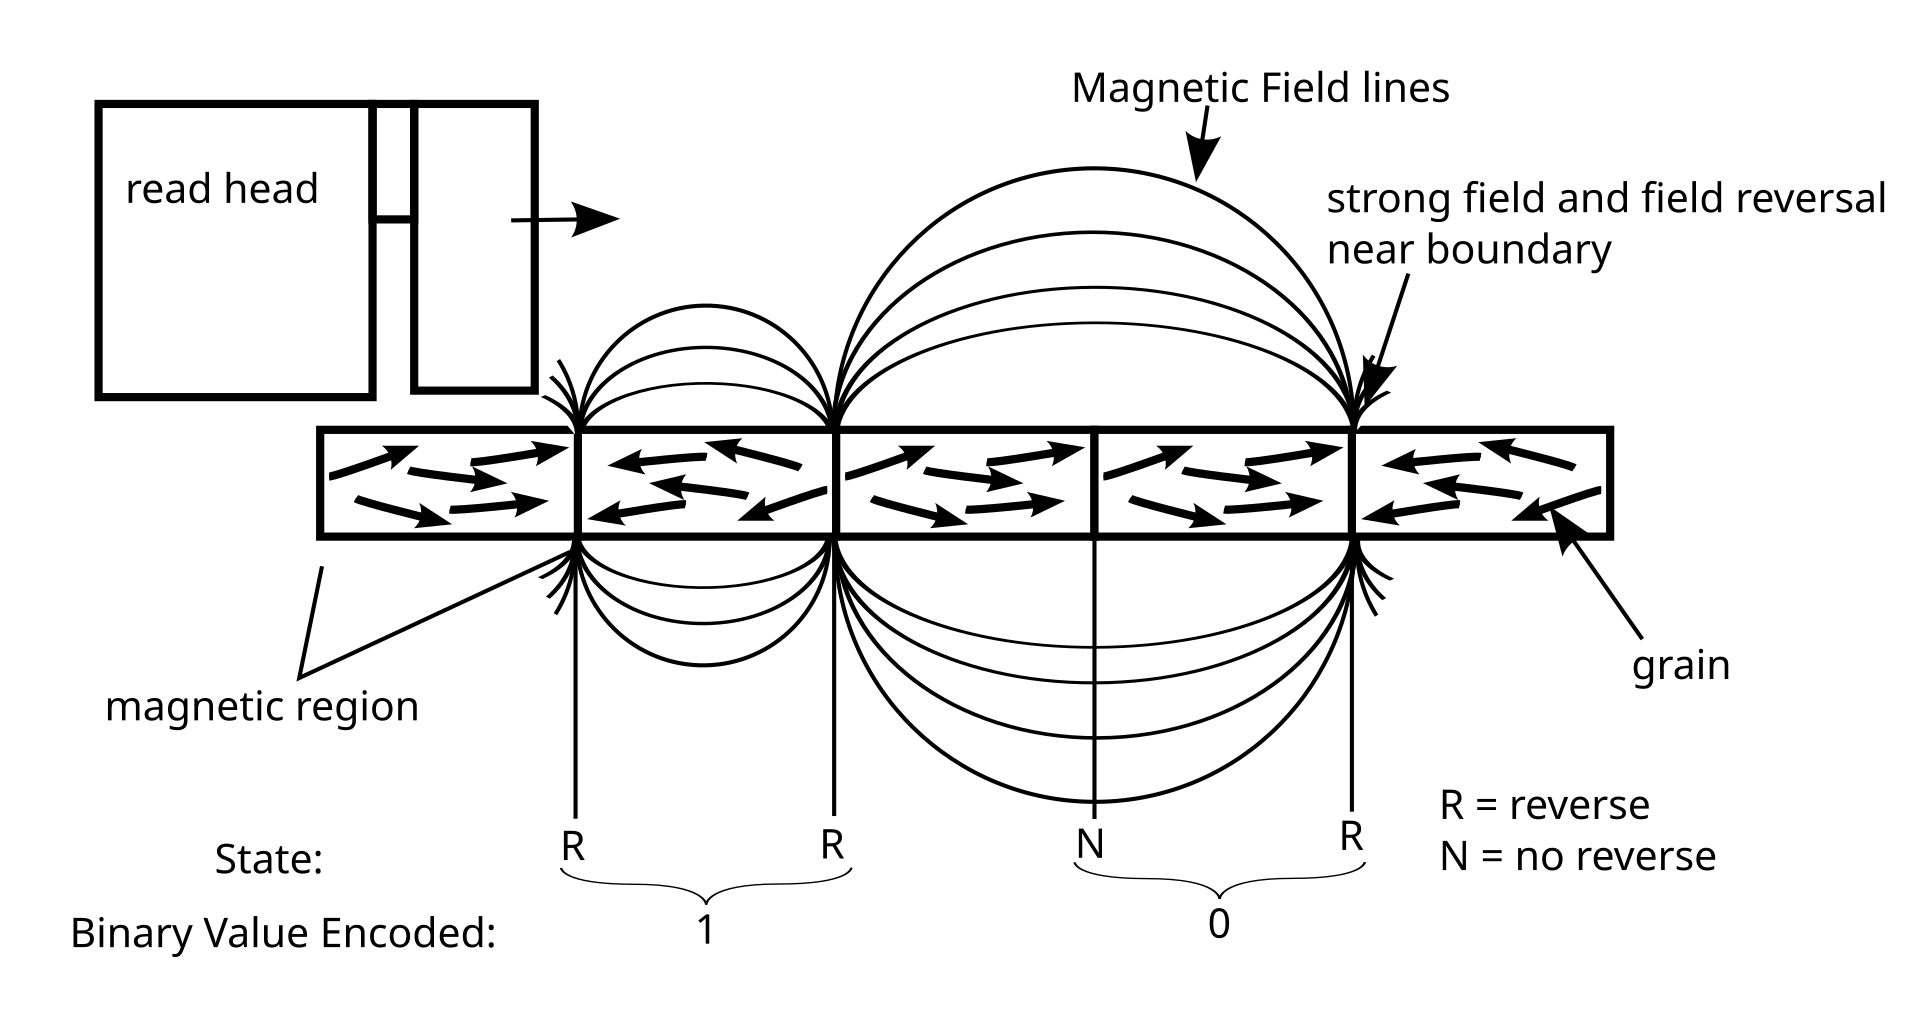
\includegraphics[width=\textwidth]{o}
\end{frame}

\begin{frame}
  \frametitle{Pevný disk (HDD)}
  \begin{minipage}{0.5\textwidth}
    \begin{itemize}[label=\textbullet]
      \item Velikost je se základem 1000 $\rightarrow$ 1 GB = 1 000 MB = 1 000 000 KB = 1 000 000 000 B, ale většina operačních systému používají základ 1024, proto se 1TB disk v počítači objeví jako disk s kapacitou 931 GB.
    \end{itemize}
    \hfill
  \end{minipage}
  \hfill
  \begin{minipage}{0.45\textwidth}
    \begin{figure}
      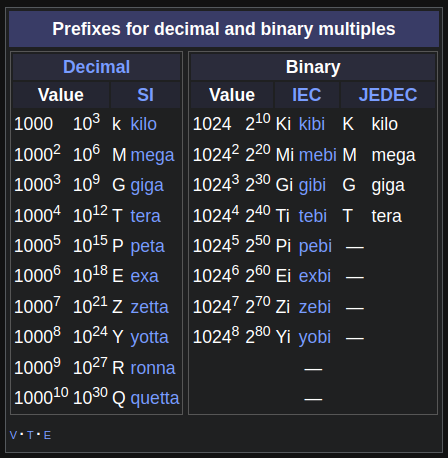
\includegraphics[width=\textwidth]{p}
      \caption{jednotky jsou confusing}
    \end{figure}
  \end{minipage}
\end{frame}
\begin{frame}
  \frametitle{Sektory disku}
  \begin{minipage}{0.45\textwidth}
    \begin{itemize}[label=\textbullet]
      \item Disk se dělí na sektory, cylindry (nebo také stopy), bloky a clustery.
      \item Blok je nejmenší jednotka, na kterou lze zapsat data.
      \item Data, které se nevejdou do jednoho bloku, zapíšou se do clusteru.
      \item Clustery jsou po obvodu, protože se disk točí, a tím pádem se čtecí hlavička nemusí pohybovat.
    \end{itemize}
  \end{minipage}
  \hfill
  \begin{minipage}{0.45\textwidth}
    \centering
    \includegraphics[width=\textwidth]{ř}
  \end{minipage}
\end{frame}
\section{Optické paměti}
\subsection{CD}
\begin{frame}
  \frametitle{\textbf{C}ompact \textbf{D}isc - 1982}
  \begin{itemize}[label=\textbullet]
    \item Optický disk.
    \item Philips a Sony.
    \item Data se nachází na jedné dlouhé spirále vedoucí ze středu.
    \item Délka spirály je zhruba 6 km. 
    \item Průměr 12 cm (může být i menší), tloušťka $1,2 mm$.
    \item Příčný odstup stopy ve spirále je $1,6 \mu m$
    \item Pro čtení kompaktních disků se používá laserové světlo s vlnovou délkou $785 nm$.
    \item Nejprve sloužilo pouze pro ukládání zvuku.
    \item Nabízí místo pro 74 minut nekomprimovaného stereo zvuku, neboli 650 MB.
    \item CD-R, CD-RW. R $\rightarrow$ recordable, RW $\rightarrow$ rewritable.
    \item Rychlost přenosu dat prvního CD byla 153,6 kB/s. Rychlost novějších modelů se udává v násobcích 153,6.
  \end{itemize}
\end{frame}

\begin{frame}
  \begin{figure}[t]
    \centering
    \begin{minipage}[t]{0.45\textwidth}
      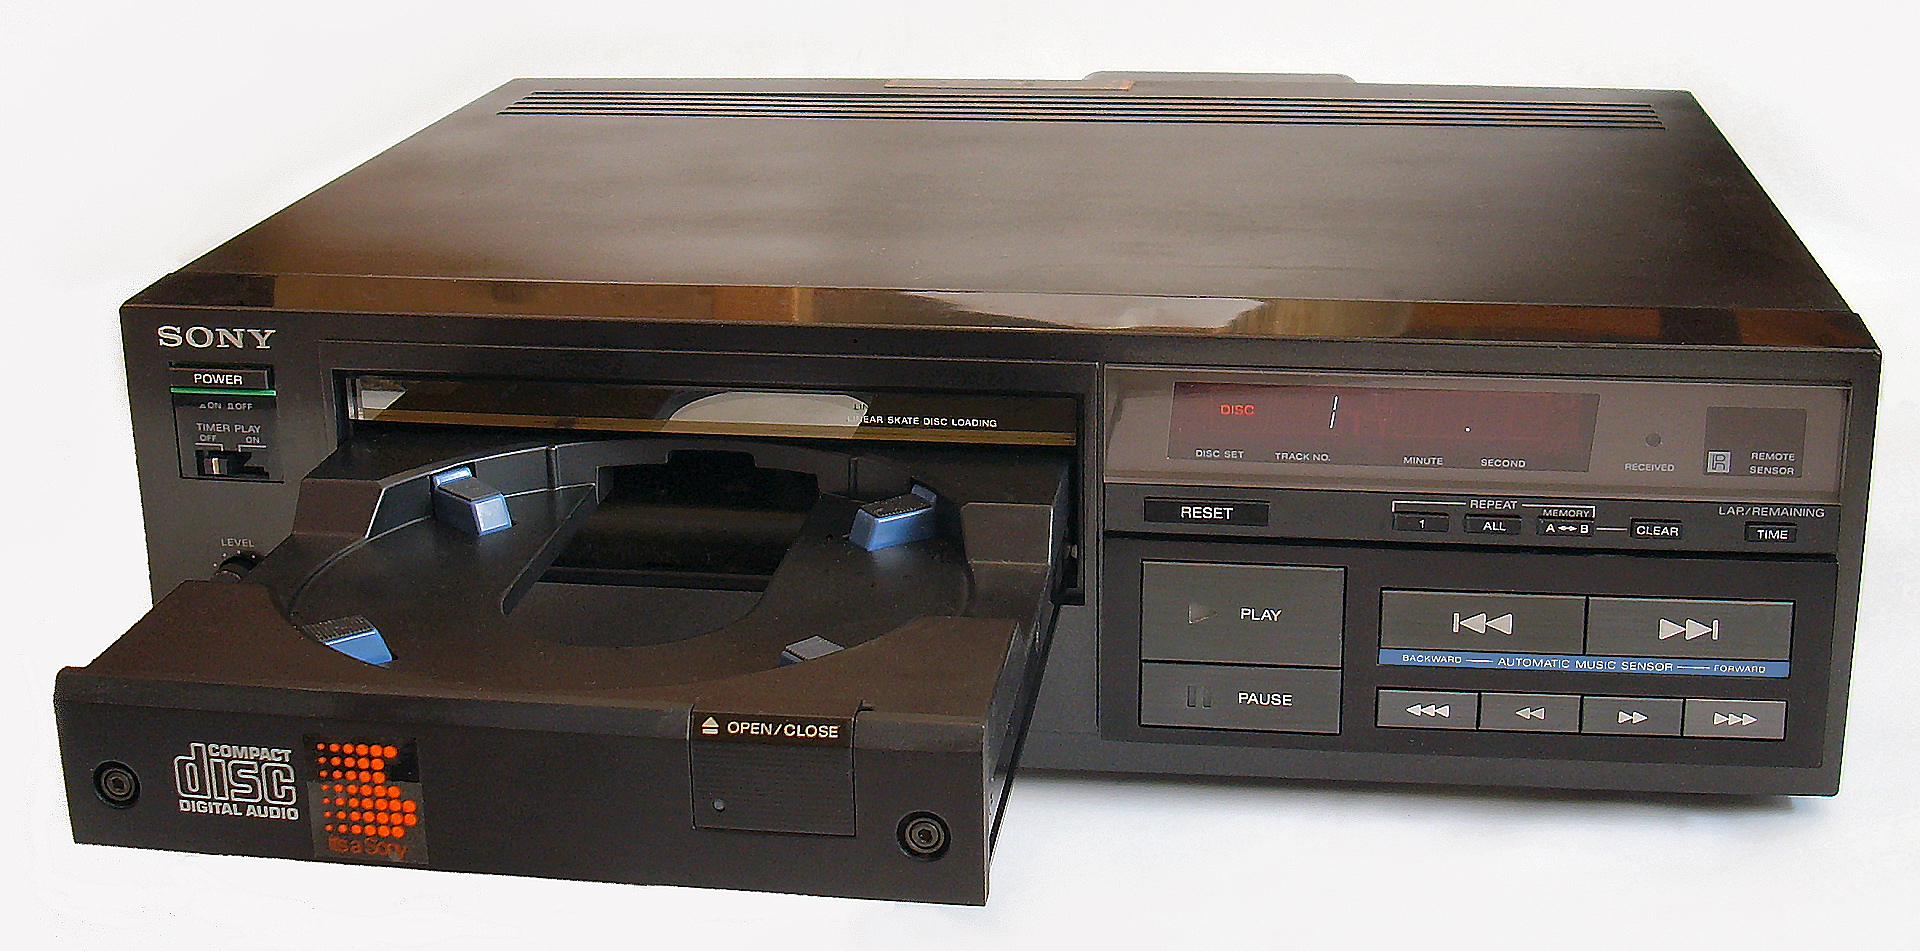
\includegraphics[width=\textwidth]{i}
      \caption{První komerčně prodávaná disková mechanika Sony CDP-101 (1982)}
    \end{minipage}
    \hfill
    \begin{minipage}[t]{0.5\textwidth}
      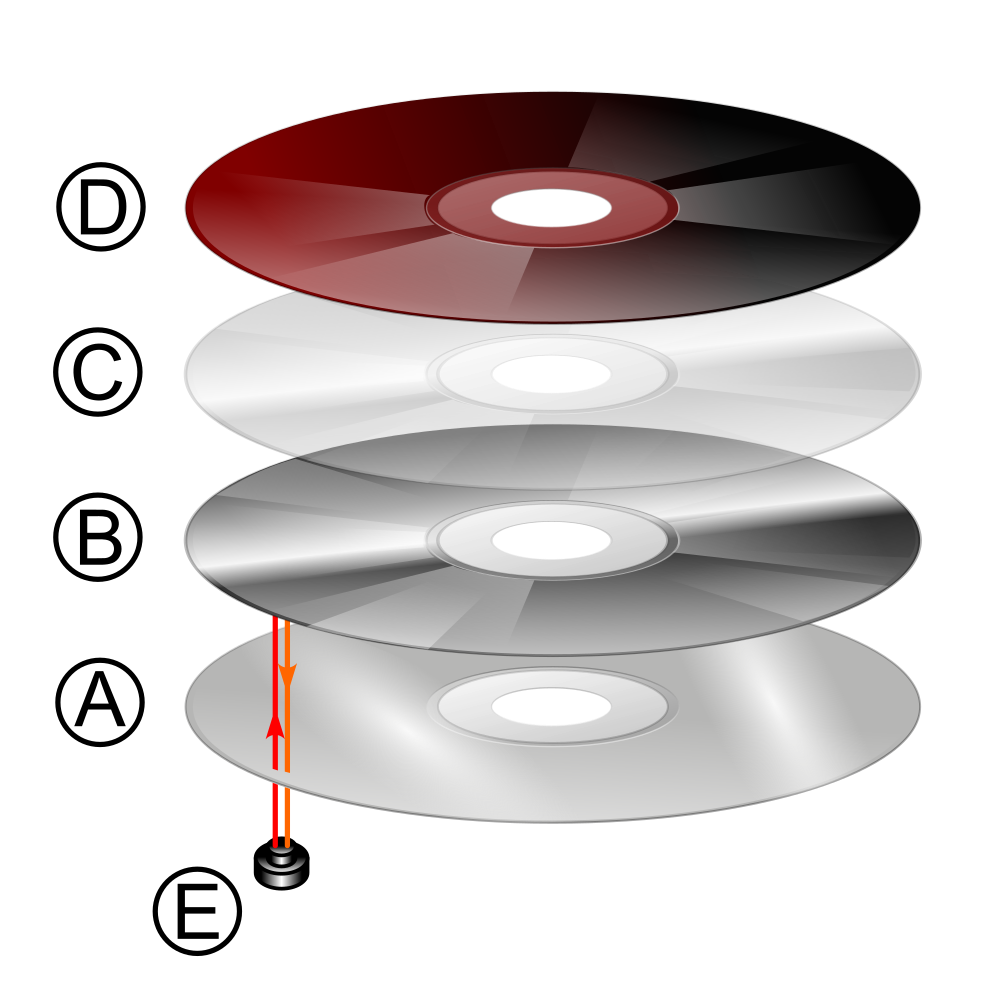
\includegraphics[width=0.7\textwidth]{h}
      \caption{A - Polykarbonátová vrstva disku má data zakódována pomocí hrbolků.  
      B - Lesklá vrstva odráží laser.  
      C - Vrstva laku chrání lesklou vrstvu.  
      D - Na horní straně disku je sítotiskem vytištěno grafické zpracování.  
      E - Laserový paprsek je odražen z CD na senzor, který jej převádí na elektronická data.}
    \end{minipage}
  \end{figure}
\end{frame}

\begin{frame}
  \begin{figure}
    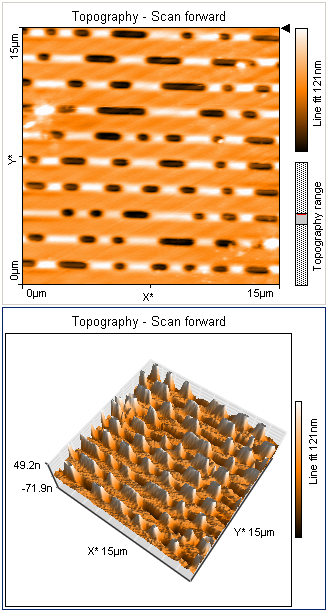
\includegraphics[width=0.25\textwidth]{k}
    \caption{Data v CD}
  \end{figure}
\end{frame}


\subsection{DVD}
\begin{frame}
  \frametitle{DVD - Japonsko 1996}
  \begin{itemize}[label=\textbullet]
    \item Philips a Sony
    \item Velmi podobný s CD.
    \item Zpětná kompatibilita s CD.
    \item Nabízejí mnohem vyšší kapacitu oproti CD.
    \item Mohou uchovávat jakékoliv data, nejčastěji ale videa.
    \item Jednostranné, pro vyšší kapacitu jsou i dvouvrstvé a oboustranné, které mohou uchovávat až 17,08 GB.
    \item DVD$\pm$R, DVD$\pm$RW R $\rightarrow$ recordable, RW $\rightarrow$ rewritable.
    \item DVD + R/RW $\rightarrow$ DVD+RW Alliance $\rightarrow$ Dell, Hp, \dots ~soupeřili s Philips a Sony.
    \item Degradují, mají životnost kolem 30 let.
    \item Rychlost přenosu dat prvního DVD byla 1,385 kB/s. Rychlost novějších modelů se udává v násobcích 1,385. Nejvyšší přenosová rychlost je 24$\times$, což je 33,2 MB/s.
  \end{itemize}

  
\end{frame}

\begin{frame}
  \begin{table}[h!] % This reduces the size of the text
    \centering
    \begin{tabular}{|c|c|c|c|c|c|}
    \hline
    \multicolumn{2}{|c|}{\textbf{Ozančení}} & \textbf{Strany} & \textbf{Vrstvy} & \textbf{Průměr (cm)} & \textbf{Kapacita (GB)} \\
    \hline
    DVD-1   & SS SL & 1& 1 & 8  & 1.46  \\
    DVD-2   & SS DL & 1& 2 & 8  & 2.65  \\
    DVD-3   & DS SL & 2& 2 & 8  & 2.92  \\
    DVD-4   & DS DL & 2& 4 & 8  & 5.31  \\
    DVD-5   & SS SL & 1& 1 & 12 & 4.70  \\
    DVD-9   & SS DL & 1& 2 & 12 & 8.54  \\
    DVD-10  & DS SL & 2& 2 & 12 & 9.40  \\
    DVD-14  & DS SL+DL & 2& 3 & 12 & 13.24 \\
    DVD-18  & DS DL & 2& 4 & 12 & 17.08 \\
    \hline
    \end{tabular}
    \caption{Specifikace DVD-R\\SS = single-sided, DS = double-sided, SL = single-layer, DL = dual-layer}
    \end{table}
\end{frame}

\subsection{Blu-ray}
\begin{frame}
  \frametitle{Blu-ray - 2005 (Japonsko)}
  \begin{minipage}{0.5\textwidth}
    \begin{itemize}[label=\textbullet]
      \item Sony a Philips.
      \item \uv{Lepší DVD}.
      \item Optický disk.
      \item Polykarbonát.
      \item Kapacita: 25 GB - 1 vrstva, 50 GB / 66 GB - 2 vrstvy, 100 GB / 128 GB - 3 vrstvy
    \end{itemize}
    \hfill
  \end{minipage}
  \hfill
  \begin{minipage}{0.45\textwidth}
    \begin{figure}
      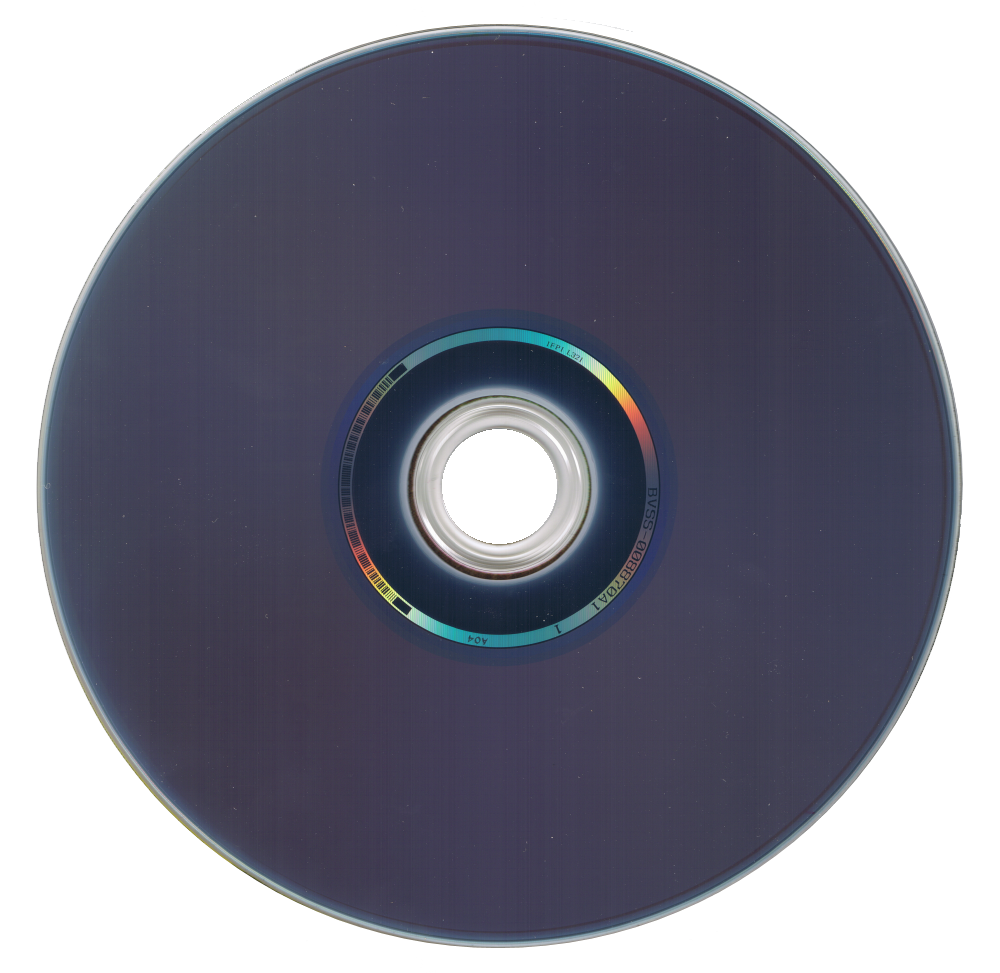
\includegraphics[width=\textwidth]{q}
      \caption{Blu-ray má modrý odraz}
    \end{figure}
  \end{minipage}
\end{frame}

\subsection{Porovnání}
\begin{frame}
  \frametitle{Porovnání CD, DVD, HD DVD, Blu-ray}
  \begin{minipage}{\textwidth}
    \includegraphics[width=0.9\textwidth]{j}
  \end{minipage}
\end{frame}


\section{Flash paměti}
\begin{frame}
  \frametitle{Flash paměť}
  \begin{minipage}{0.5\textwidth}
    \begin{itemize}[label=\textbullet]
      \item NAND nebo NOR flash.
      \item Základ je  floating gate MOSFET (metal–oxide–semiconductor field-effect transistor).
      \item Elektricky programovatelná.
      \item Organizovaná po blocích.
      \item \href{https://youtu.be/r2KaVfSH884?t=89}{Jak funguje flash paměť? (video)}
    \end{itemize}
    \hfill
  \end{minipage}
  \hfill
  \begin{minipage}{0.45\textwidth}
    \begin{figure}
      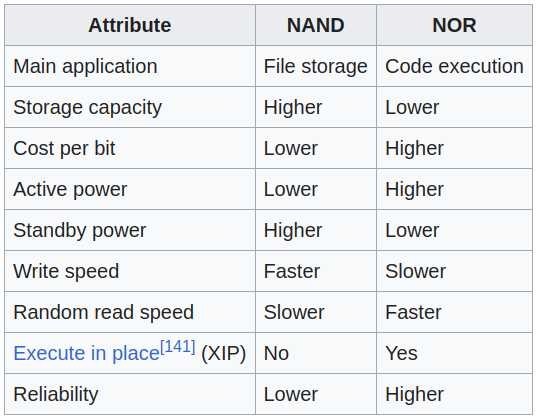
\includegraphics[width=\textwidth]{w}
      \caption{Rozdíly mezi NAND a NOR}
    \end{figure}
  \end{minipage}
\end{frame}

\begin{frame}
  \frametitle{Flash paměť}
  \begin{minipage}{0.45\textwidth}
    \begin{figure}
      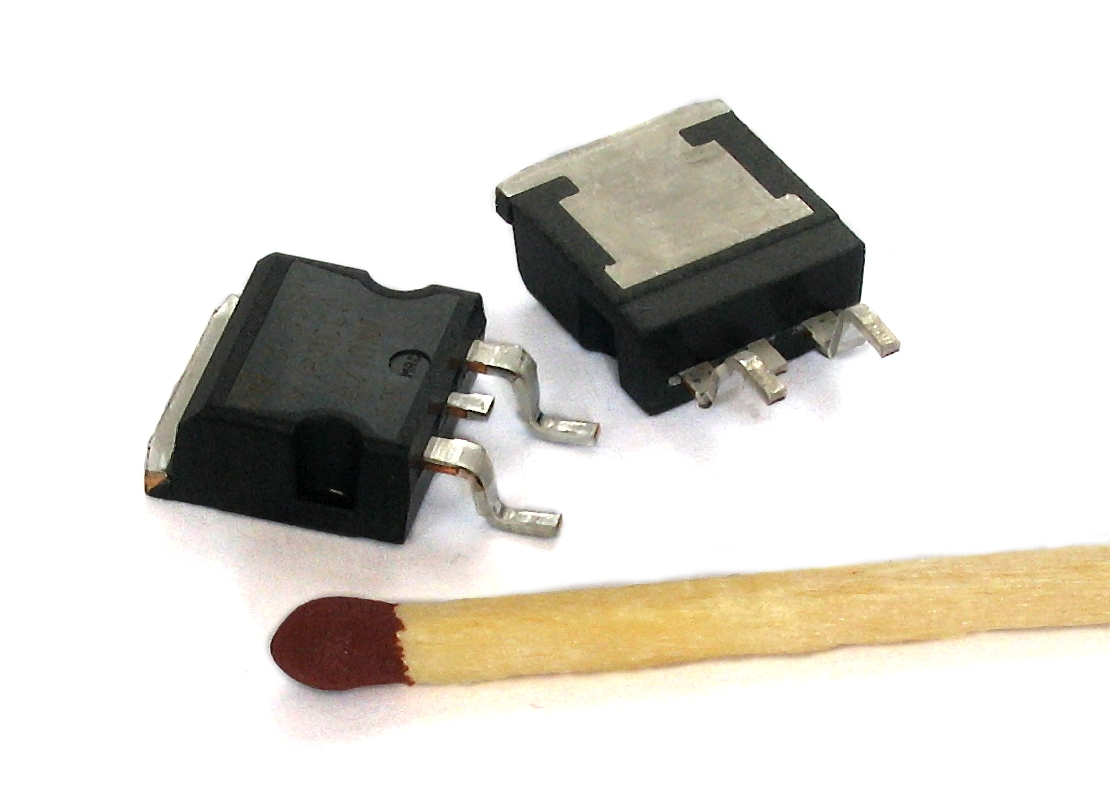
\includegraphics[width=\textwidth]{x}
      \caption{MOSFET}
    \end{figure}
  \end{minipage}
  \hfill
  \begin{minipage}{0.45\textwidth}
    \begin{figure}
      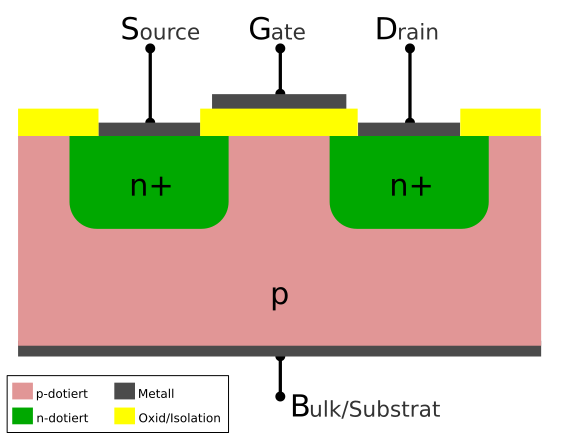
\includegraphics[width=\textwidth]{y}
      \caption{diagram MOSFET}
    \end{figure}
  \end{minipage}

\end{frame}




\subsection{SSD}
\begin{frame}
  \frametitle{SSD - 1991 (SanDisk)}
  \begin{minipage}{0.5\textwidth}
    \begin{itemize}[label=\textbullet]
      \item Většinou 2$\times$ dražší, než HDD.
      \item Různe typy: SATA, PCIe, NVMe, M.2.
      \item Nemá žádné pohyblivé části.
    \end{itemize}
    \hfill
  \end{minipage}
  \hfill
  \begin{minipage}{0.45\textwidth}
    \begin{figure}
      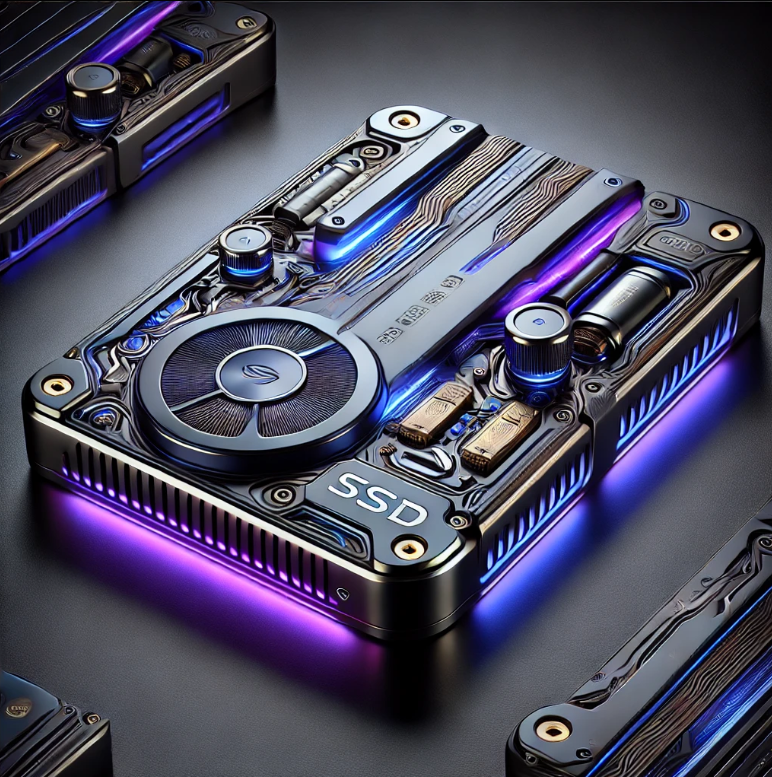
\includegraphics[width=\textwidth]{s}
      \caption{Nejhezčí SSD podle AI}
    \end{figure}
  \end{minipage}
\end{frame}
\begin{frame}
  \begin{figure}
    

  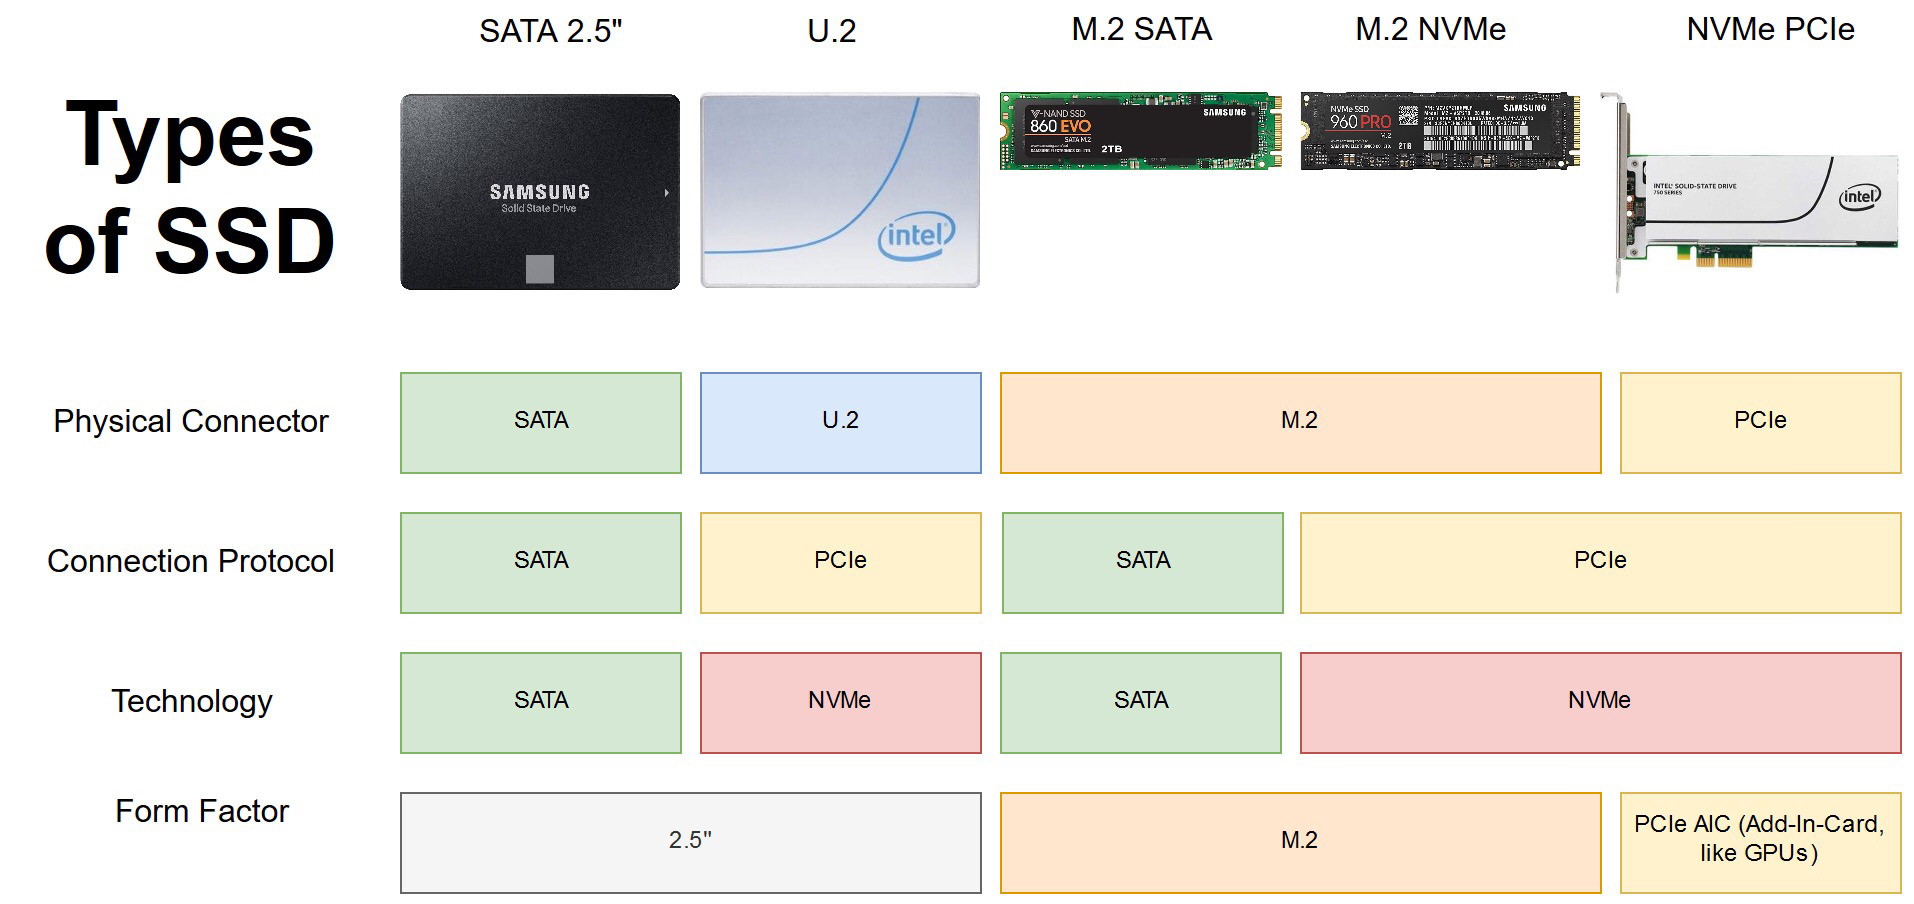
\includegraphics[width=\textwidth]{t}
  \caption{Všechno je to confusing}
\end{figure}
\end{frame}
\begin{frame}
  \frametitle{SATA III vs mSATA vs M.2 (podrobný popis z Alzy)}
  \begin{itemize}[label=\textbullet]
    \item SATA III je již silně zažité rozhraní pro připojení interních disků. Moderní SSD disky však rychlostně překonávají možnosti sběrnice SATA, která využívá komunikační rozhraní AHCI optimalizované především pro mnohem pomalejší HDD.
\item mSATA je jakýmsi duchovním předchůdcem formátu SSD disků M.2. Z názvu vyplývá, že komunikuje pomocí sběrnice SATA, takže se na tento formát vztahují veškerá její omezení. Výhodou jsou pouze menší rozměry. Netěší se přílišné popularitě a se standardními konektory SATA není kompatibilní, proto raději dvakrát zkontrolujte, zda váš počítač tímto specializovaným slotem disponuje.
    \item M.2 je moderní formát, díky kterému mohou SSD disky nabývat úspornějších rozměrů. Namísto montování do pozic ve skříni se tato úložiště umisťují přímo na základní desku. Formát M.2 otevírá nové rychlostní možnosti pro SSD disky, což zajišťuje především s ním kompatibilní rozhraní NVMe.
  \end{itemize}
\end{frame}
\begin{frame}
  \frametitle{2,5“ vs PCI-Express vs U.2. (podrobný popis z Alzy)}
  \begin{itemize}[label=\textbullet]
    \item 2,5“ je tradiční formát přejatý od starších plotnových disků. Tyto SSD disky nejsou drahé a hodí se i do starších sestav či notebooků, protože se připojují přes zavedenou sběrnici SATA III. Moderním způsobem připojení rychlejších 2,5“ SSD disků je také port U.2.
  \item PCI-Express SSD disky využívají standardní NVMe řadič, pouze se připojují skrze obecný port PCIe x4, kterým disponují prakticky všechny základní desky. Pro M.2 SSD disky lze zakoupit redukční adaptér pro PCIe slot.
  \item U.2. Formát M.2 umožnil SSD disky výrazně zmenšit, což v některých aplikacích omezilo jejich kapacitu. Konektor U.2 dokáže připojit 2,5“ SSD disky pomocí standardu NVMe a zajistit tak vysoké rychlosti i pro ně. Pokud vaše základní deska konektorem U.2 nedisponuje, lze ho skrze redukci připojit do slotu M.2.
  \end{itemize}
\end{frame}

\subsection{USB flash disk}
\begin{frame}
  \frametitle{USB flash disk - 2000 (IBM a Trek Technology)}
  \begin{minipage}{0.5\textwidth}
    \begin{itemize}[label=\textbullet]
      \item První flashky měly kapacitu 8 MB.
    \end{itemize}
    \begin{figure}
      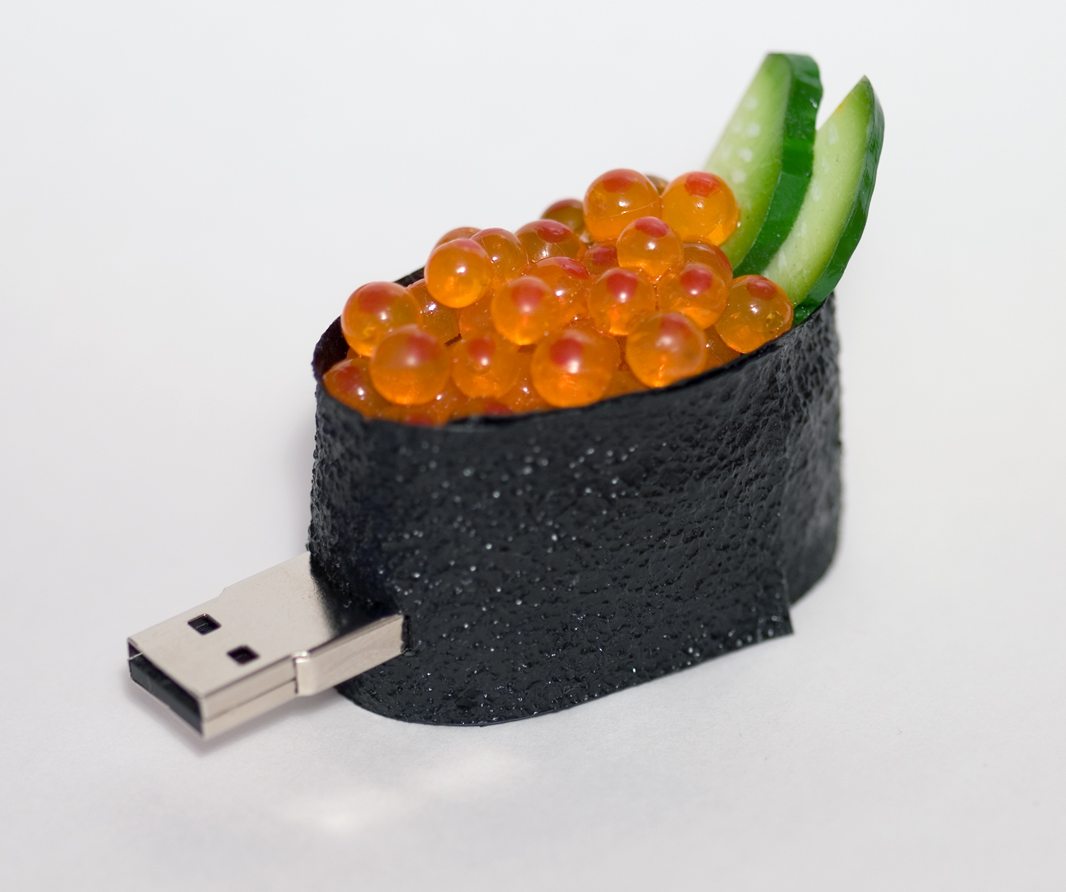
\includegraphics[width=0.7\textwidth]{Sushiusb}
      \caption*{SushiUSB}
    \end{figure}
  \end{minipage}
  \hfill
  \begin{minipage}{0.45\textwidth}
    \begin{figure}
      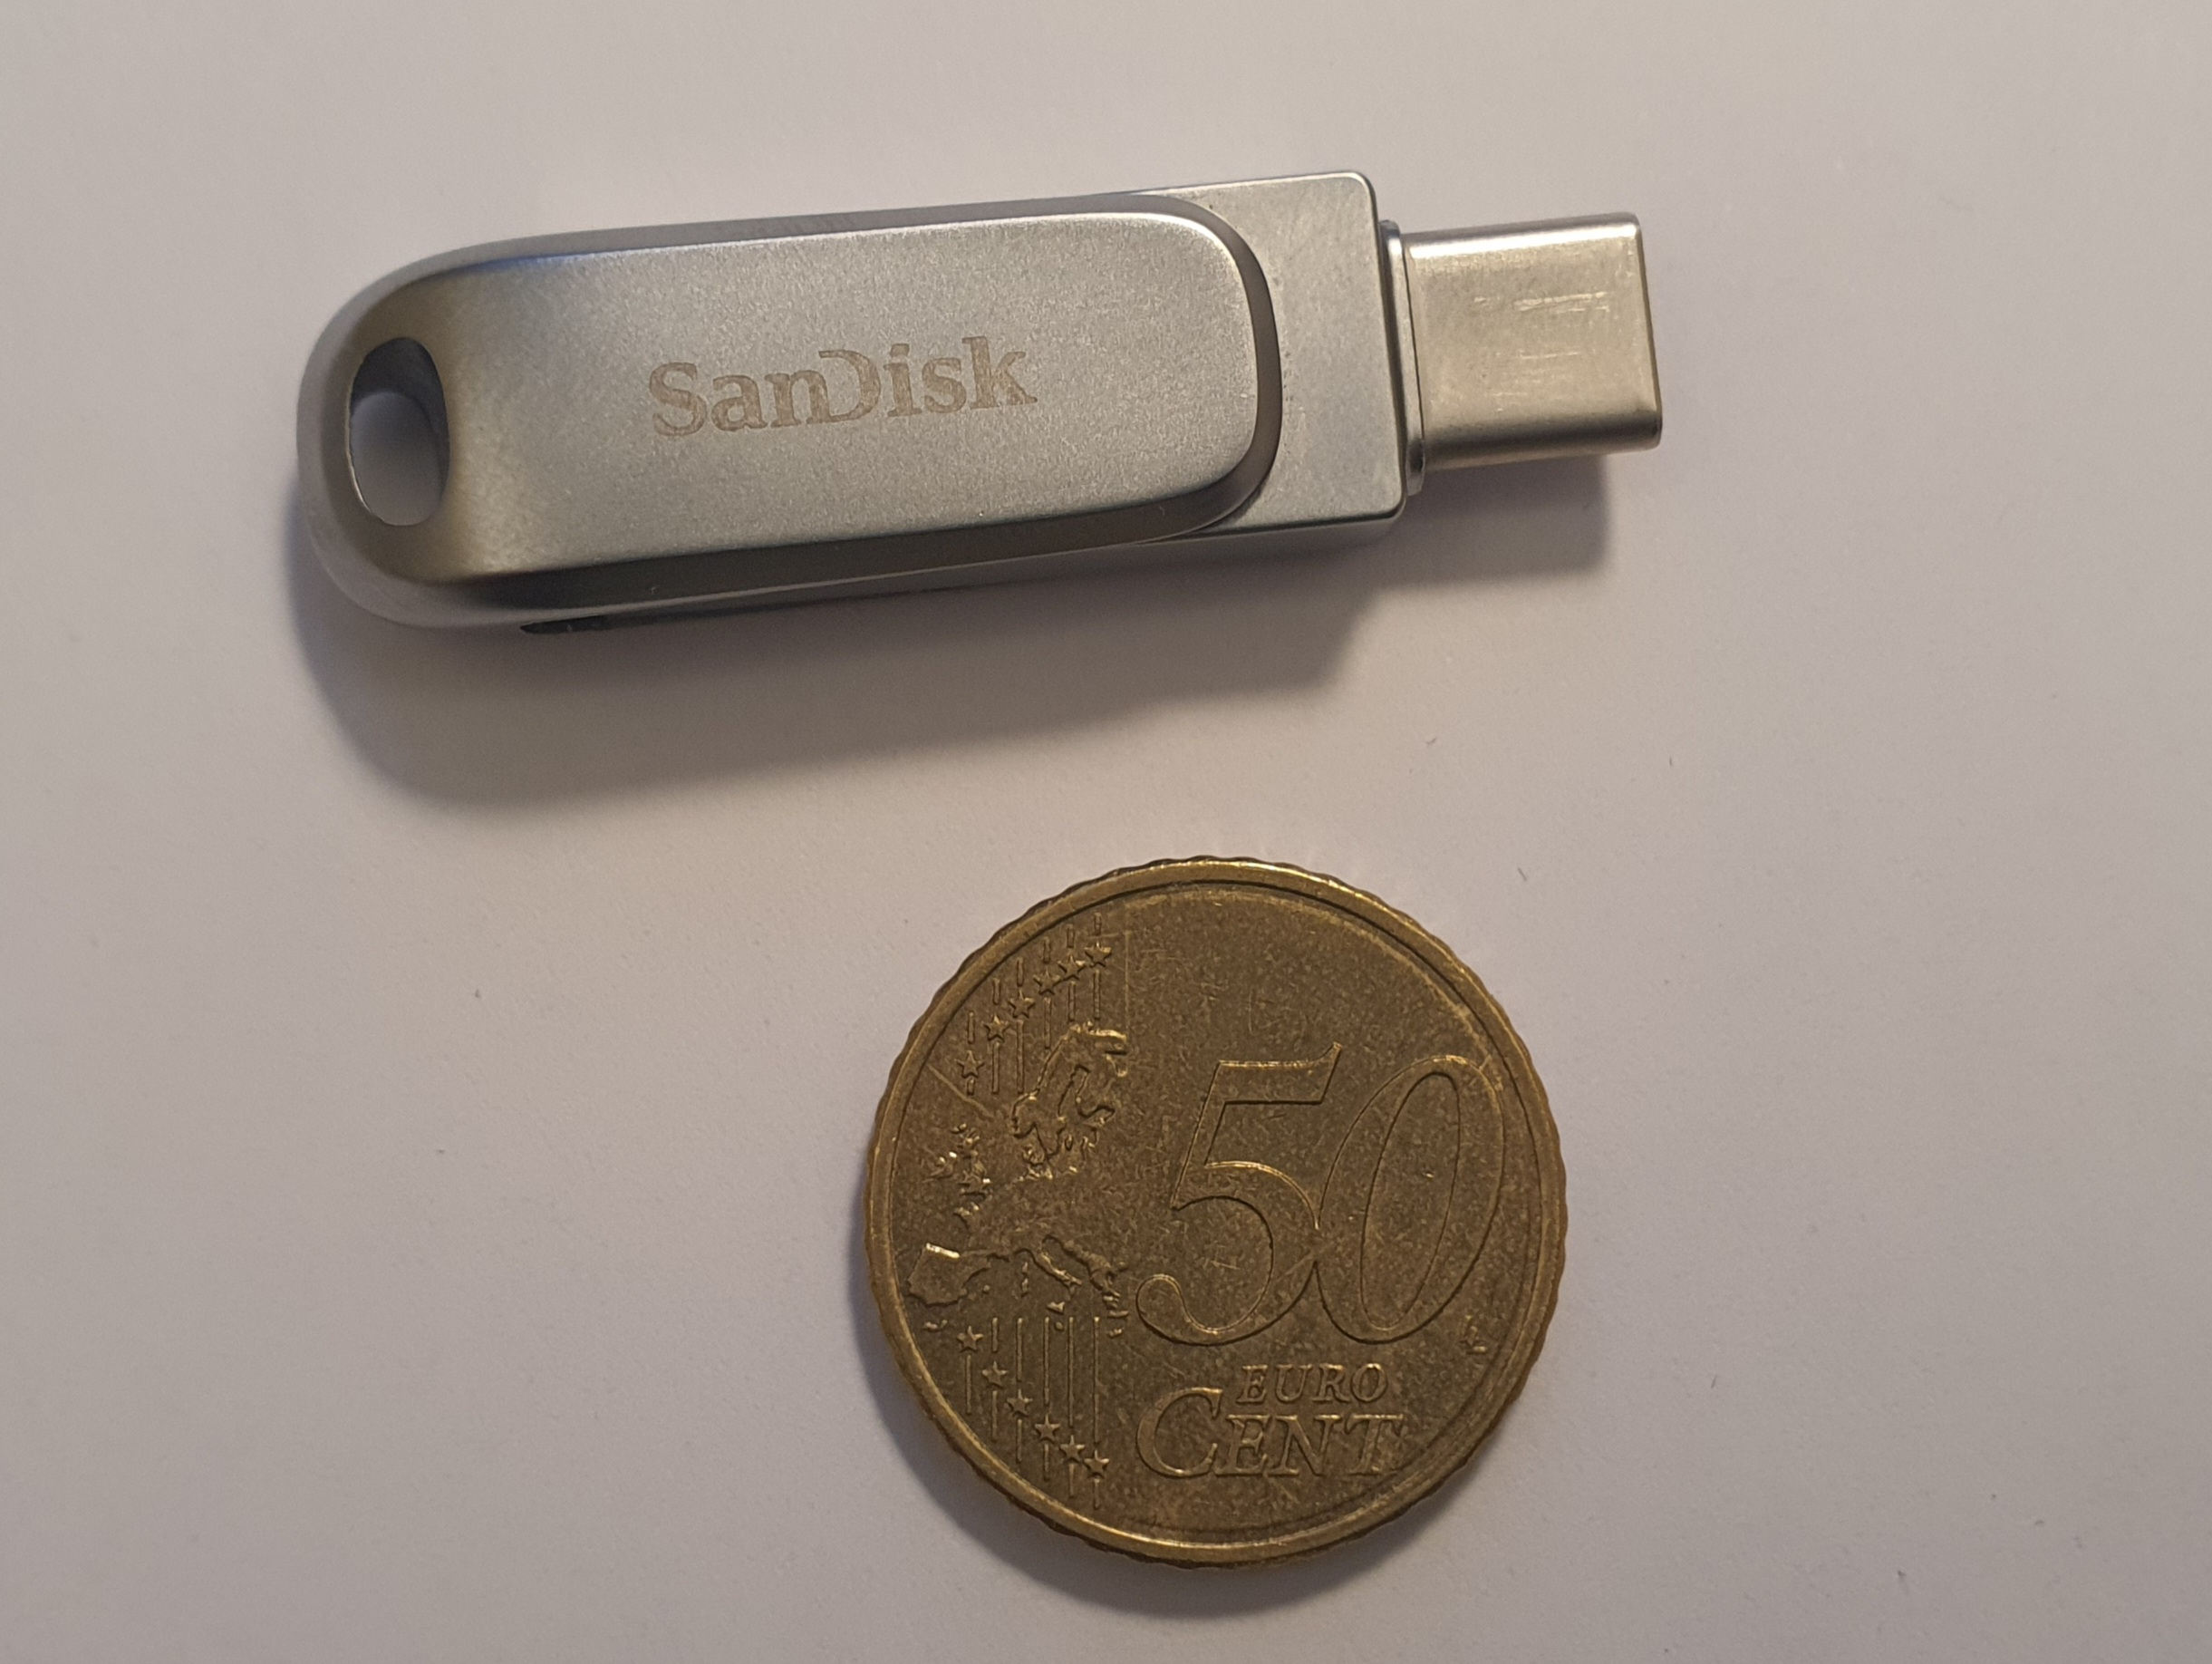
\includegraphics[width=\textwidth]{v}
      \caption{USB-C 1 TB flashka}
    \end{figure}

    
  \end{minipage}
\end{frame}
\begin{frame}
  \frametitle{Rozbor USB flashky}
  \begin{minipage}{0.5\textwidth}
    \begin{itemize}[label=\textbullet]
      \item 1 - USB Standard-A, "male" plug
      \item 2 -	USB mass storage controller device
      \item 3	- Test point
      \item  4 -	Flash memory chip
      \item 5	- Crystal oscillator
      \item  6 -	LED (Optional)
      \item 7	- Write-protect switch (Optional)
      \item 8	- Space for second flash memory chip
    \end{itemize}
    \hfill
  \end{minipage}
  \hfill
  \begin{minipage}{0.45\textwidth}
    \begin{figure}
      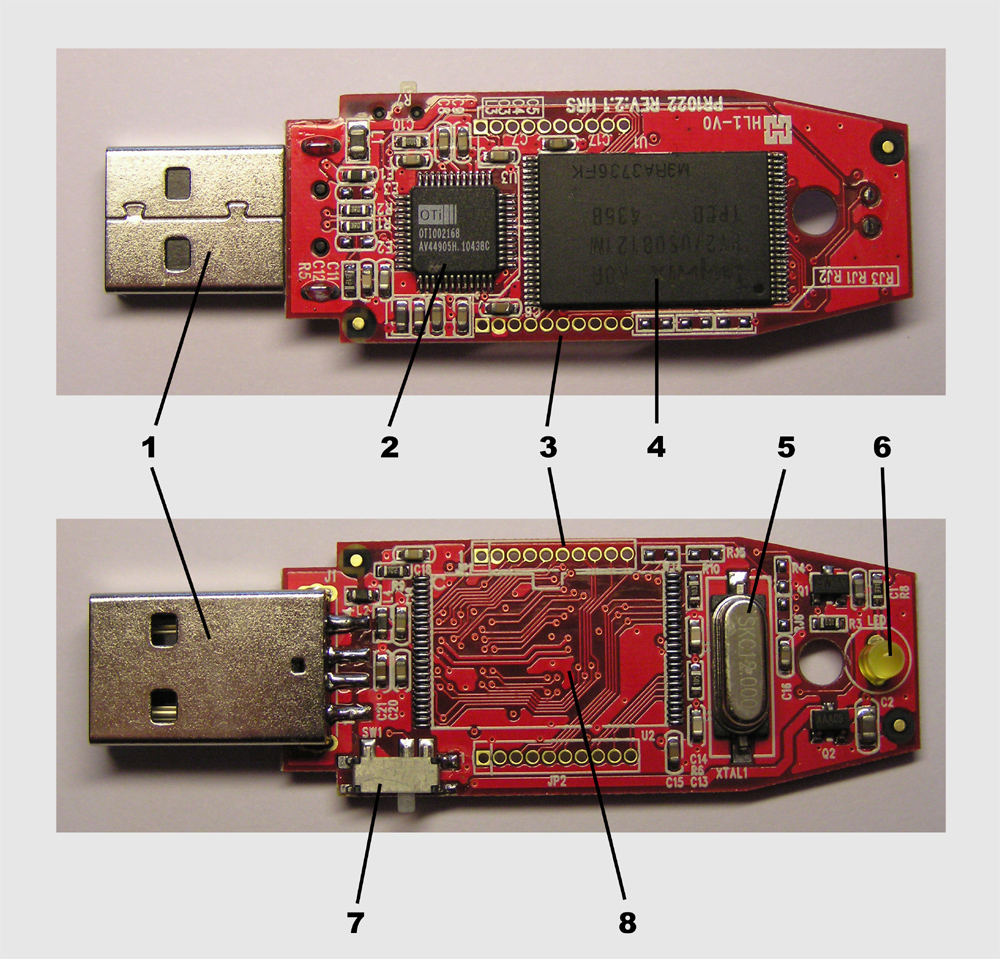
\includegraphics[width=\textwidth]{u}
    \end{figure}
  \end{minipage}
\end{frame}

\subsection{SD karty}
\begin{frame}
  \frametitle{SD karty - 1999 (SanDisk, Panasonic, Toshiba)}
  \begin{minipage}{0.5\textwidth}
    \begin{itemize}[label=\textbullet]
      \item Secure Digital (SD) karty jsou populární formou flash paměti.
      \item Používají se v digitálních fotoaparátech, mobilních telefonech, tabletech a dalších zařízeních.
      \item Kapacita se pohybuje od několika MB až po 1 TB.
      \item Různé formáty: SD, miniSD, microSD.
      \item Rychlostní třídy: Class 2, 4, 6, 10, UHS-I, UHS-II, UHS-III.
    \end{itemize}
    \hfill
    \tiny (tento slide vytvořil github copilot)
  \end{minipage}
  \hfill
  \begin{minipage}{0.45\textwidth}
    \begin{figure}
      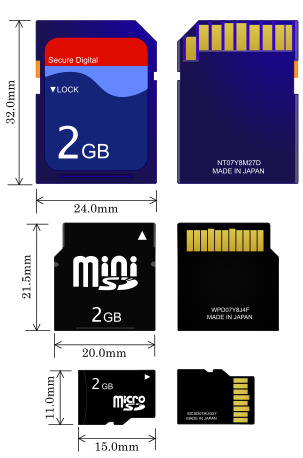
\includegraphics[width=0.5\textwidth]{z}
      \caption{Různé typy SD karet}
    \end{figure}
  \end{minipage}
\end{frame}
\begin{frame}
  \frametitle{Konec}
\end{frame}
\end{document}